%& --shell-escape
\documentclass[letterpaper, 12pt]{report}
\usepackage[utf8]{inputenc}
\usepackage[english, spanish]{babel}
\usepackage{fullpage} % changes the margin
\usepackage{graphicx} 
\usepackage{amsmath}
\usepackage{enumitem} 
\usepackage{chngcntr}
\usepackage{setspace}
\usepackage{url}
\counterwithin{figure}{section}
\renewcommand{\thesection}{\arabic{section}} 
\renewcommand{\thesubsection}{\thesection.\arabic{subsection}}
\renewcommand{\baselinestretch}{1.5}
\usepackage{float}
\usepackage{verbatim}
\usepackage{apacite}
\bibliographystyle{apacite}
\setlength\belowcaptionskip{10pt}
\linespread{1.5}

\begin{document}

\begin{titlepage}
	\centering
	
\includegraphics[width=0.3\textwidth]{Images/logo_utb.png}\par\vspace{1cm}
	{\scshape\LARGE Universidad Tecnológica de Bolívar \par}
	\vspace{1cm}

	{\scshape\Large FÍSICA ELÉCTRICA \par}
	\vspace{.2cm}

	% chktex-file 8
	{\scshape\Large H1 - C \par}
	\vspace{1cm}
	% chktex-file 8
	\slshape {\Large \bfseries{} LAB 4 -   \\}
	\vspace{1cm}

	\slshape {\itshape{} Mauro González, T00067622 \\}
	\slshape {\itshape{} German De Armas Castaño, T00068765 \\}
	\slshape {\itshape{} Angel Vega Rodriguez, T00068186 \\}
	\slshape {\itshape{} Juan Jose Osorio Ariza, T00067316 \\}
	\slshape {\itshape{} Juan Eduardo barón, T00065901 \\}
	\vfill
	Revisado Por \\
	Gabriel Hoyos Gomez Casseres\\
	{\large \today\par}
\end{titlepage}

% ----------------------------------------------------------------------|>
\section{Introducción}

La ley de Ohm es una ley fundamental en la física eléctrica que establece la
relación entre la corriente eléctrica, el voltaje y la resistencia en un
circuito eléctrico. Fue formulada por el físico alemán Georg Simon Ohm en
1827 y se utiliza ampliamente en la ingeniería eléctrica para diseñar y
analizar circuitos.

\bigskip

Establece que la corriente que fluye a través de un conductor
es directamente proporcional al voltaje aplicado e inversamente proporcional
a la resistencia del conductor. Esta relación se expresa matemáticamente como
I = V/R, donde I es la corriente eléctrica en amperios, V es el voltaje
en voltios y R es la resistencia en ohmios.

\bigskip

Es fundamental para entender el comportamiento de los circuitos
eléctricos y es la base de muchas otras leyes y teoremas eléctricos.
Además, es esencial para el diseño y análisis de circuitos eléctricos
en una amplia variedad de aplicaciones, desde la electrónica de consumo
hasta la energía eléctrica industrial.

\bigskip

Esta cuarta experiencia se enfocará en hallar la resistividad de un conductor
o su resistencia especifica además de conocer y diferenciar el comportamiento
de materiales óhmicos y no óhmicos.

\begin{figure}[H]
	\begin{center}
		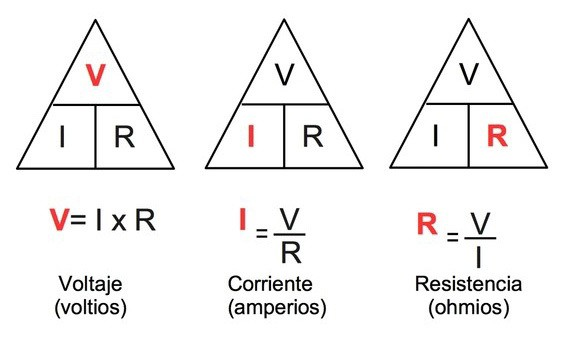
\includegraphics[scale = 0.5]{./Images/LeyDeOhm.jpg}
	\end{center}
\end{figure}

\newpage

% ----------------------------------------------------------------------|>
\section{Objetivos}

\subsection{Objetivos Generales}

\newpage

% ----------------------------------------------------------------------|>
\section{Preparación de la practica}

% ------------------------------------------------------------|>
\subsection{Ley de Ohm}

Según la ley de Ohm, la cantidad de corriente que fluye a través de un
conductor es proporcional a la cantidad de voltaje aplicada a través de
él. Esta ley fue descubierta experimentalmente por el físico alemán Georg
Simon Ohm a principios del siglo XIX, quien demostró que la corriente que
fluye a través de un material conductor es directamente proporcional a la
diferencia de potencial eléctrico a través del mismo. El descubrimiento de
Ohm fue fundamental en el desarrollo de la idea de resistencia en los
circuitos eléctricos.~\cite{LeyDeOhm}

% ------------------------------------------------------------|>
\subsection{Materiales Óhmicos}

Son sustancias que se conocen con el nombre de resistencias lineales;para estas
resistencias se cumple que, la diferencia de potencial entre sus extremos es
proporcional a la corriente que circula por ella; esto quiere decir que la
resistencia es independiente de la tensión y la corriente, cumpliendo de esta
manera con la ley de ohm, V = IR.\@ Dentro de los materiales óhmicos tenemos:
los conductores metálicos.~\cite{MaterialesOhmicos}

% ------------------------------------------------------------|>


% ------------------------------------------------------------|>
\subsection{Factores en los que depende la resistencia y resistividad de un
	material}

% -----------------------------------------------|>
\subsubsection*{Resistencia}

La oposición que presentan los cuerpos se debe a que los electrones al moverse
en el interior de los átomos rozan produciendo choques que desprenden energía
en forma de calor. Cuanto mayor es el número de choques, mayor es la
resistencia que presenta el material.

\begin{itemize}
	\item La sección del elemento conductor (a mayor sección menor resistencia)
	\item La longitud del mismo (a mayor longitud, mayor resistencia)
	\item La naturaleza del conductor, sabemos que hay materiales que dejan
	      pasar muy bien la corriente y otros que no. La característica que
	      define la mayor o menor oposición del material al paso de la corriente
	      es la resistividad.
\end{itemize}

La resistividad r se mide en $[\Omega \cdot mm^2 /m]$.

Estos tres factores se relacionan con la resistencia mediante la siguiente
ecuación:

\smallskip

$R = \rho \cdot \frac{l}{S}$

\smallskip

Donde $\rho$ es la resistividad en $[\Omega \cdot mm^2 /m]$, l la longitud
en $[M]$ y S la sección en $[mm^2]$.

Tomado de:~\cite{ResistenciaElectrica}

% -----------------------------------------------|>
\subsubsection{Resistividad}

La resistividad $\rho$ de un material depende de la estructura molecular y
atómica, y es dependiente de la temperatura. Para la mayoría de los
conductores, la resistividad aumenta con el aumento de temperatura.
~\cite{KhanAcademyResistividad}

% ------------------------------------------------------------|>
\subsection{Temperatura relacionada a la resistividad y resistencia de
	un material}

% -----------------------------------------------|>
\subsubsection{Resistencia}

Uno de los efectos perjudiciales del efecto Joule es el
calentamiento que se produce en los conductores eléctricos
cuando son recorridos por una corriente eléctrica. Para evitar
que este calentamiento alcance valores que sean perjudiciales
para los mismos se construyen de diferentes secciones. Cuanto
más corriente se prevé que va fluir por ellos, mayor será su sección.

\bigskip

La sección de un conductor es la superficie que aparece
cuando le cortamos perpendicularmente a su longitud. Por lo
general los conductores son cilíndricos, por lo que la sección
suele ser un área circular. La sección de los conductores
se suele expresar en $mm^2$

\bigskip

Dado que los conductores no son perfectos y poseen una
cierta resistencia eléctrica, cuando son atravesados por
una corriente eléctrica se producen dos fenómenos:

\begin{itemize}
	\item Se calientan y pierden potencia.
	\item Al estar conectados en serie con los aparatos eléctricos
	      que alimentan, se produce una caída de tensión, que
	      hace que se reduzca notablemente la tensión, al final
	      de la línea.
\end{itemize}

\bigskip

Estos son los dos factores más importantes que hay que
tener en cuenta a la hora de seleccionar la sección más adecuada para una
instalación eléctrica.

\bigskip

Si se aplica la misma diferencia  de potencial entre los extremos de una
barra de cobre y de una barra de madera  se producen corrientes muy diferentes.
La característica del conductor que  interviene en esta diferencia es su
resistencia.

\smallskip

Tomado de:~\cite{TemperaturaResistencia}

% -----------------------------------------------|>
\subsubsection{Resistividad}

\begin{itemize}
	\item La resistividad es casi nula a temperaturas próximas al 0 absoluto.
	\item En los metales y aleaciones, la resistividad aumenta con la
	      temperatura: a mayor temperatura, mayor resistividad, y por tanto,
	      menor conductividad. Estas variaciones son siempre positivas para los
	      metales y sus aleaciones.
\end{itemize}

\smallskip

Tomado de:~\cite{TemperaturaResistividad}

% ------------------------------------------------------------|>
\subsection{Gráfica de Voltaje vs. Corriente}

\begin{figure}[H]
	\begin{center}
		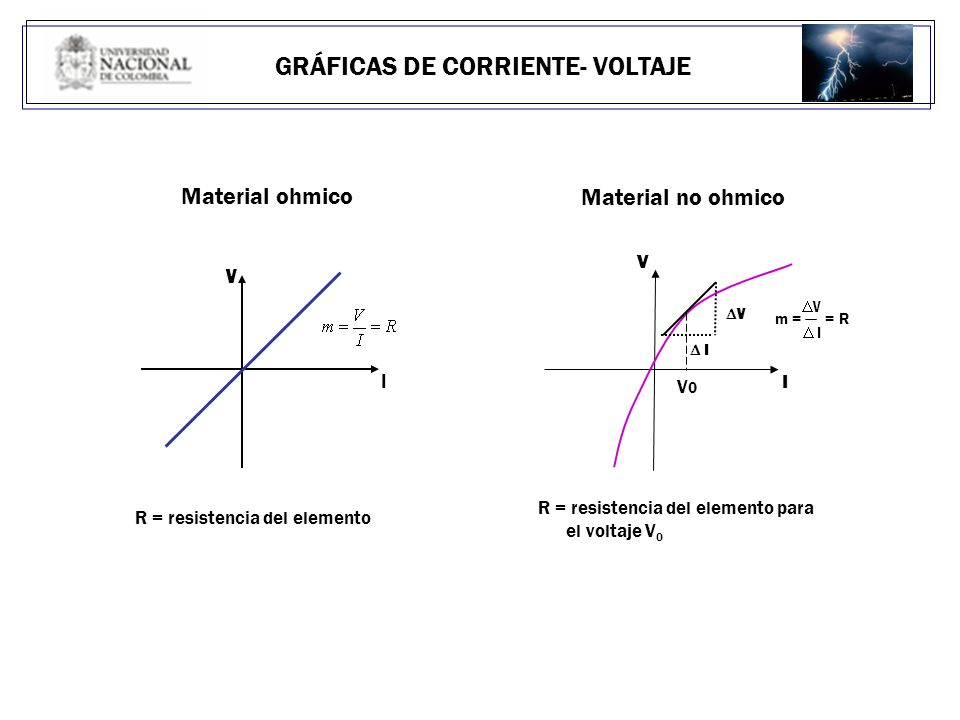
\includegraphics[scale = 0.5]{./Images/VoltajeVsResistencia.jpg}
		\caption{Gráfico de Voltaje vs. Corriente}
		% chktex-file 24
		\label{img:graficoResistencias}
	\end{center}
\end{figure}

Tomado de:~\cite{GraficaVoltajeCorriente}

% ------------------------------------------------------------|>
\subsection{Calcular la resistencia a partir del gráfico Voltaje vs.\hfill{}
	\break{} Corriente}

Analizando las gráficas (\ref{img:graficoResistencias}), es muy notorio como en el caso de los materiales
óhmicos, la resistencia aumenta constantemente a lo largo del gráfico. En
otras palabras, la resistencia es inversamente proporcional a la corriente
(Intensidad). Esto quiere decir que el valor de la resistencia en ese punto
esta dado por:

$R = \frac{V}{I}$

\vspace{.5cm}

Mientras que para los materiales no óhmicos, la resistencia esta
dada por:

$R = \frac{\triangle V}{\triangle I}$, siendo la pendiente $[m]$ el valor
de la resistencia para un voltaje $V_0$.

% ----------------------------------------------------------------------|>
\section{Resumen del procedimiento}


\newpage
\bibliography{./Bibliography/bibliography.bib}

\end{document}